\chapter{Memory}

\begin{center}
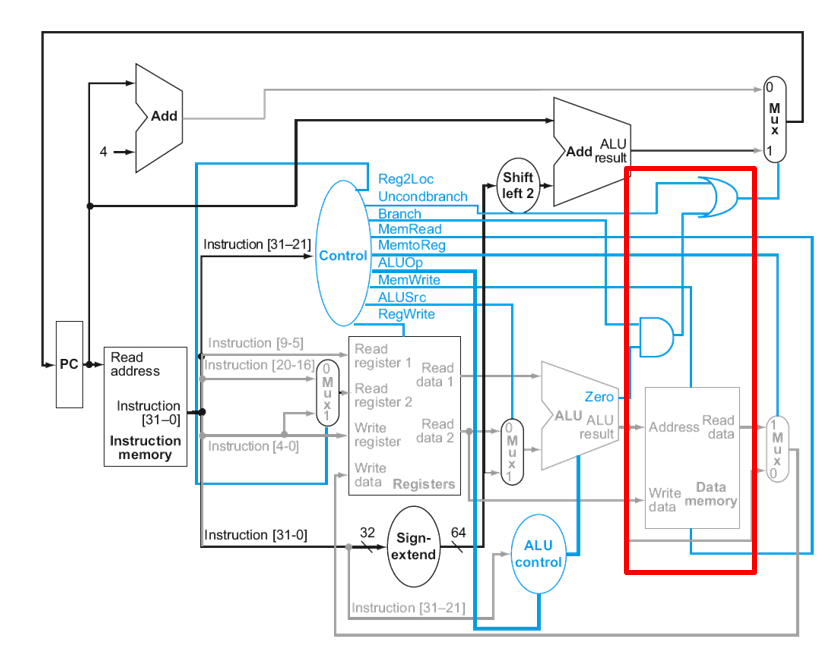
\includegraphics[width=5.5in]{../images/data_memory.png}
\end{center}

\section{Memory Stage}
Today we will create the iMemory stage of our processor.  This stage contains the data memory for the system that we use for load and store commands.  It also contains the logic gates used to produce the pc\_src signal that is used in the iFetch stage.  Note that although the diagram shows the pc\_src mux on the right side of the diagram, the mux is actually already implemented in the iFetch stage and belongs in the iFetch stage.

\section{Branch Resolution}

We now have all the information necessary to decide if the computer should branch or not.  We have the signal `branch' to tell us if it is a branch command, and we have `zero' to tell us if the condition was met.  Both branch and zero must be true so we will combine them with an `and' gate.

We also need an 'or' gate to 'or' together the output of the branch 'and' gate (above) and the uncondBranch control signal.  These gates can be included in your iMemory module as one line commands.  They do not need to be explicity tested, as they will be thoroughly tested when we integrate the system.  

\section{Data Memory}

This will be almost exactly like the instruction memory, with only two changes:
\begin{enumerate}
\item reading is now conditional on the MemRead' control wire being high.
\item writing is now permissible if the MemWrite' control wire is high.
\end{enumerate}
As such, take your instruction memory (it is the right size, you could also use your register memory, but that would require more modification) and add the two changes above then test.

\section{Your Assignment}

You are to:
\begin{enumerate}
\item Create a new module called iMemory.
\item Instantiate the AND and OR gates directly in the iMemory stage.
\item Use instruction memory as a basis for a data memory module, and add the two new changes.  Also create or modify a ramData.data file.
\item Integrate data memory into the iMemory stage.  
\item Write a testbench to verify that the iMemory stage works properly. Use a combination of ramData.data and testbench to test various scenarios.
\item We will not write a full lab report for this lab.  Instead, we will submit a simplified report that will just allow me to make sure that everyone is making good progress.  Write a simplified lab report in LaTex that includes:
\begin{enumerate}
	\item  A one paragraph intro describing your results.  Please indicate whether the modules worked properly or not.  If you have any other comments that you want me to know, please put them here.
	\item Your module code, test bench code, and simulation results for each module created.  You do not need to add additional text in this section unless there is something that you want to communicate to me.
\end{enumerate} 
\end{enumerate} 